\documentclass[pdflatex,sn-mathphys-num]{sn-jnl}% Math and Physical Sciences Numbered Reference Style

\renewenvironment{table}[1][]%
{\tableorg[#1]%
\tablebodyfont%
\renewcommand\footnotetext[2][]{{\removelastskip\vskip3pt%
\let\tablebodyfont\tablefootnotefont%
\hskip0pt\if!##1!\else{\smash{$^{##1}$}}\fi##2\par}}%
}{\endtableorg}

\usepackage{graphicx}%
\usepackage{multirow}%
\usepackage{amsmath,amssymb,amsfonts}%
\usepackage{amsthm}%
\usepackage{mathrsfs}%
\usepackage[title]{appendix}%
\usepackage{xcolor}%
\usepackage{textcomp}%
\usepackage{manyfoot}%
\usepackage{booktabs}%
\usepackage{algorithm}%
\usepackage{algorithmicx}%
\usepackage{algpseudocode}%
\usepackage{listings}%
\usepackage{natbib}%

\usepackage{tikz} 
\usetikzlibrary{positioning}
\definecolor{darkred}{rgb}{0.7, 0, 0}
\usepackage{pifont} % \ding{55} for xmark

\raggedbottom


\begin{document}

% page header
\title[Article Title]{Mitigating environmental uncertainty of autonomous vehicles via shortest-paths in digraph models}
\author[1]{\fnm{Amr} \sur{El Mougy} (corresponding author)}\email{amr.elmougy@aucegypt.edu}
\author[1]{\fnm{Sherif} \sur{Aly}}\email{sgamal@aucegypt.edu}
\author[3]{\fnm{Daoud} \sur{Siniora}}\email{daoud.siniora@aucegypt.edu}
\author[1]{\fnm{Mostafa} \sur{Touny}}\email{mostafa.touny@aucegypt.edu}
\affil[1]{\orgdiv{Computer Science and Engineering}, \orgname{The American University in Cairo}, \orgaddress{\country{Egypt}}}
\affil[2]{\orgdiv{Mechanical Engineering}, \orgname{The American University in Cairo}, \orgaddress{\country{Egypt}}}
\affil[3]{\orgdiv{Mathematics and Actuarial Science}, \orgname{The American University in Cairo}, \orgaddress{\country{Egypt}}}


\abstract{Uncertain environments exert additional challenges to the safety of autonomous vehicles. An example of such an unpredictable element is object detection error. Mitigation techniques include multi-sensor data integration, motion planning, and risk assessment. Upon accommodating multiple scenarios and environments, challenges arise due to scalability concerns and the additional work incurred by building a module for each distribution. We propose a graph-theoretic framework, modeling uncertainty as a vector of random variables for a subset of vertices. The probabilistic expected harm is reduced to finding a shortest path. Neutral digraph zones are queried by a faster subroutine, to reduce the computational time on uncertain zones. Besides correctness proofs, tested emulations on Carla show a reduction in harm caused.}

\maketitle

\newpage

\section{Introduction}

Autonomous vehicles are a central pillar of many workflows in various industries. Yet, safety remains a critical bottleneck of its widespread adoption in public roads. The issue has social and regulatory implications as well. It is crucial to foster public trust, and address communication and transparency among stakeholders. A safe navigation relies on predictable environment alongside accurate sensors' data. Any unexpected environmental events or inaccuracies in sensors endanger people's lives. Understanding their sources, how they affect safety, and mitigating them is crucial for system's robustness and reliability.

Those unpredictable elements include: weather conditions like rain, snow, fog, and strong winds; Dull lightning conditions; Terrains variations like slopes; Sensors noise as for example in LiDARs by signals distortion in fog; Dynamic movements of objects like vehicles and pedestrians whereby vehicles may take sudden lane changes or stops, and pedestrians may move in an unusual or unpredictable way \cite{alharbi2020global}. Technically, uncertainty could be in misclassifying objects, inaccurate positioning, unpredictable trajectories, or in sudden appearance of objects. The focus of this paper is in the first two categories of uncertainties.

If a decision-making mechanism doesn't consider uncertainty, then this could clearly lead to unacceptable paths. A child may be hit because it is misclassified as a plastic bag \cite{tahir2024object}. A planner may hit an object due to distance measurements inaccuracies \cite{itkina2022uncertainty} whereby an object is reported to be more faraway than its actual position. If the mechanism aims to avoid uncertainty by being more conservative, then it is likely to complicate the path to avoid any potential threat. In some cases, a path avoiding all uncertainty may not be existing. Even if it exists, it needs to resolve more constraints incurring more computational time.

These uncertainties necessitate algorithms and modeling techniques capable of reasoning under uncertainty. Ongoing efforts in the literature include: Multi-sensor data integration \cite{vargas2021overview} where it addresses the limitations of individual sensors, such as Global Navigation Satellite Systems (GNSS) inaccuracies in urban canyons or LiDAR in adverse weather conditions, by merging data from various sensors; Motion planning \cite{tang2022driving} where new developments are in path density adjustments and the integration of hierarchical motion planning methods; Risk assessment \cite{wang2021risk} where a risk index is estimated based on various indicators like visibility and the presence of obstructions, allowing for dynamic updates in decision-making strategies; Probabilistic optimization frameworks \cite{han2022non} where the uncertainty of environmental conditions and obstacles are modeled. Those enable algorithms to generate risk-bounded decisions minimizing the likelihood of undesirable actions, as in trajectory planning.

In an environment, some factors are completely known with total confidence, while others are uncertain. Their unpredictability degrees could range from low to high in the same environment. In practice, optimizing for these multiple degrees of uncertainty often requires considering each distribution or scenario separately, solving each with a distinct solution. For example, in \cite{OnboardMitigation_2} the planner is designed to be conservative to handle perception errors. The bounding boxes of all objects, regardless of perception accuracy, are enlarged. Similarly in \cite{OnboardMitigation_3}, an estimation or assumption of the perception uncertainty is required. In \cite{OnboardMitigation_4} an uncertainty adaptive planner is designed to estimate the degree of uncertainty. Therefore, in order to accommodate different distributions, and environmental factors, in a single module, a hybrid approach is frequently employed, where specialized models or methods are combined to handle various smaller sub-problems. However, the hybrid approach introduces several drawbacks: Scalability issues arise \cite{scalabilityML} because the complexity of the solution increases as multiple specialized solutions are integrated, to account for more factors or constraints; Additional time and cost are incurred due to designing, implementing, testing, and maintaining multiple models. More efforts are required for the integration and maintainability of the system as a whole; Reduced interpretability \cite{UncertainSurvey}, as it is more difficult to analyze or explain decision-making processes, based on multiple specialized solutions working together. Tracing would require analyzing each specialized module and how their outcomes are combined to produce the end result; Moreover, The effectiveness of data-driven models heavily depends on the quality of available datasets, as poor or biased data won't result in a robust agent. So accommodating multiple distributions and scenarios shall raise the concern of finding quality datasets for the whole case-study in hand; The trade-off among multiple objectives and scenarios in hybrid solutions requires a careful tuning on behalf of the designer, as favoring one objective could tamper others.

In this work, we tackle object misclassification and inaccurate positioning uncertainties. We adopt graph theoretic modeling of the environment, where the vehicle's decision is a path over the digraph, computed algorithmically. It is independent of any particular scenario, dataset, environment knowledge. We choose probabilistic expectation as a quantitative measure for the path planning in uncertain environments. It captures both the likelihood of objects classification alongside associated penalties of their priorities to the planner. For instance, it is natural to assign hitting pedestrians a greater penalty than hitting inanimate objects like a banner. The linearity of expectation allows us to compute the total expected risk of a path by summing uncertain zones' expectations the path navigates through. It aligns well with traditional shortest path algorithms, which evaluate path weights by summing the costs of the vertices they traverse. Our solution reduces computational time by treating differently uncertain zones and neutral zones devoid of uncertainty. A faster subroutine is used for the latter, so that expensive shortest path queries are exclusive on uncertain regions.

Algorithmic correctness is proved using graph theory and logic techniques. Empirical emulation is based on dropout sampling, whereby a decision is taken according to a probability distribution over the digraph, then we emulate the decision on a sampled digraph, corresponding to the environment. Emulations are on Carla open-source simulator for autonomous driving research.

Carla's waypoints correspond to vertices, and probabilities correspond to vertices' weights. Implementation is by Carla's built-in basic agent module \cite{py-carla}. Carla's built-in path planning modules were not used as more waypoints are needed within two-adjacent road segments. A simple Python script is written to construct a digraph from Carla's waypoints.


\section{Outline}

We start with basic graph-theory and probability notation. We recall some useful properties of graphs' adjacency matrices. In Section \ref{Modeling}, we illustrate how graph-theoretic notions and vertices weights do capture the external uncertain environment of autonomous vehicles. We prove the equivalence of some scenarios with respect to probabilistic expectation. In Section \ref{Algorithm} we illustrate our framework from a higher-level view, showing how uncertain subgraphs are connected to neutral subgraphs. Then we give more details of subroutines. Namely, reducing vertex weights to edge weights, and querying a neutral path. The section ends with dynamic updates whereby a path is adjusted without recomputing everything from scratch. In Section \ref{Evaluation}, the dropout sampling methodology is explained, and how is it applied on digraph traversal. Finally, Section \ref{Experimentation} shows Carla emulation testing results on selected scenarios.

\section{Modeling} \label{Modeling}

We illustrate our framework for autonomous vehicle path planning in environments with uncertain elements. An uncertain object's diameter and probability is modeled as a subgraph with weighted edges. Navigating through uncertain conditions, minimizing total probabilistic expectation, is accounted by finding a shortest-weight path.

A vehicle's possible paths may be thought of by a set of discrete waypoints, whereby each waypoint allows the transition to some other waypoints. In terms of graph theory, it is a digraph $G$ where waypoints correspond to vertices $V(G)$, and valid transitions are given by directed edges $E(G)$. An edge $(a,b)$ indicates a transition from waypoint $a$ to waypoint $b$ is possible.

An object's uncertain classification is given by a probability distribution over classes. For example we may classify an object as either a dog with probability 0.7 or a cat with probability 0.3. Likelihoods and penalties could be combined by probabilistic expectation $Ex[X]$. For example, the expected harm or penalty is $Ex[X] = (2 \cdot 0.3) + (1 \cdot 0.7)$ given cats are twice as important or penalizing as dogs. A vertex weight $w(v)$ is set with such expectation denoting classification uncertainty.

An object's uncertain position corresponds to potential subset of vertices, which we call an uncertain subgraph $U$. Since the object is known to exist, vertices of $U$ constitute a probability distribution. For example, if an object's position may be uniformly uncertain among nearby vertices $v_1, v_2, v_3, v_4, v_5$ where $(v_1,v_2), (v_1, v_3), (v_1, v_4), (v_5,v_1) \in E(G)$. Similarly, a constant penalty, since it is the same object, may be set for all vertices of $U$.

We will prove later it is equivalent to set a weight for edge $(a,b)$ in place of vertex $b$ weight. By linearity of expectation, the total probabilistic expectation of a path is the summation of edges' weights the path navigates through. It follows, computing a shortest path suffices for minimizing the total expectation.

We are given a simple directed graph $G$. That is, a set $V$ together with an irreflexive binary relation $E$ on $V$. We call them vertices and directed edges. Our digraphs are anti-symmetric between any two vertices. The sample space $\Omega$ is the set of all possible objects at some waypoint. By convention, no two objects are present in the same waypoint, so $Pr[E] = 0$ for all $E \subseteq \Omega$ where $|E| \geq 2$. A random variable $X$ associates a penalty for each outcome, and the corresponding random variable distribution $\mu_X$ associates probabilities for outcomes.

\textbf{Definition.} For a subset of vertices $S = \{ v_1, \dots, v_k \} \subseteq V(G)$ and a set of random variable distributions $\{ \mu_{X_1}, \dots, \mu_{X_k} \}$, an \textit{uncertain zone} is a function $U$
$$
U: v_i \mapsto \mu_{X_i}.
$$

\textbf{Examples.} See \textit{Figure 1} for a visualizing aid.
\begin{itemize}
    \item \textit{Case 1.} $U = \{ (v_8, \{(1, 0.7)\} ) \}$ denotes an object is present in some vertex $v_8$ with probability $0.7$.
    \item \textit{Case 2.} $U = \{ (v_8, \{(1, 0.3)\}), (v_{12}, \{(1, 0.3)\}), (v_{14}, \{(1, 0.3)\}) \}$ denotes an object is present in one of vertices $v_8$, $v_{12}$, and $v_{14}$, each with probability $0.3$.
    \item \textit{Case 3.} $U = \{ (v_8, \{ (100, 0.5), (5, 0.5) \} ) \}$ denotes $v_8$ either has a box with probability $0.5$ and penalty $5$, or a pedestrian with probability $0.5$ and penalty $100$.
\end{itemize}

\textbf{Definition.} "given an uncertain zone" "number definitions". Since each $X$ induces $Ex[X]$ on a vertex, an \textit{uncertain environment} is declared to be a tuple $(G, h:V(G) \rightarrow \mathbb{R} )$, of a digraph $G$ and a partial function $h$ labeling vertices.

\begin{center}
  \input{figures/modeling}
  Figure 1: The environment modeled as a digraph
\end{center}

\vspace{5mm}

Observe two cases. In the former, a single object's existence is known but its position is probabilistically uniform. In the latter, it is possible to have multiple existing objects or none at all. In both cases, the expectation of a vertex $Ex[\mu_{X_i}]$ is the same. As we aim in our work to reduce the expected harm, we don't need to distinguish the former case from the latter. So a single approach enables us to solve both cases.

\textbf{Lemma.} For an uncertain zone $U$, the following two scenarios result in exactly the same expectation for vertices: (1) An object is uniformly placed into a vertex of the subgraph; (2) Each vertex independently has an object with probability 1/k.

\textit{Proof.} Let $X_i$ be an indicator random variable, taking value $1$ if an object is placed in the ith vertex and $0$ otherwise. In the first case, since the object is placed uniformly, each vertex has exactly $1/k$ probability of receiving it. In the second case, by definition, each vertex independently has probability $1/k$ of containing an object. Therefore, in both scenarios, $Pr[X_i=1] = 1/k$ for any vertex $i$. The expected value of $X_i$ is $Ex[X_i] = 1 \cdot Pr[X_i=1] + 0 \cdot Pr[X_i=0] = 1 \cdot (1/k) + 0 \cdot ((k-1)/k) = 1/k$. Thereby, despite the different underlying distribution, both scenarios yield identical expected labeling across all vertices in the subgraph.

\textbf{Proposition.} In both cases, traversing the whole subgraph, in expectation hits a single object. This means that regardless of whether we use the first method (uniformly placing exactly one object across the k vertices) or the second method (independently assigning an object to each vertex with probability 1/k), the expected number of objects encountered when examining all vertices remains the same.

\textit{Proof.} By applying the linearity of expectation property, the expected total number of objects in the subgraph is $Ex[X_1 + X_2 + \dots + X_k] = Ex[X_1] + Ex[X_2] + \dots + Ex[X_k]$. We already know $Ex[X_i] = 1/k$ for each vertex $i$, and there are $k$ vertices in total, then the expectation is $k \cdot (1/k) = 1$. While the proof is simple but the observation is counterintuitive, as the second scenario could potentially place multiple objects or no objects at all.


\section{Algorithm} \label{Algorithm}

We distinguish between uncertain subgraphs and neutral subgraphs devoid of any uncertainty. Shortest-path algorithms are queried on uncertain subgraphs. A fast subroutine searches for paths among the neutral zone, connecting those uncertain subgraphs with each other. Combining computed paths of uncertain zones and neutral zones is realized by constructing a smaller higher-level graph as in \textit{Figure (3-4)}. Finding a shortest-path of it, accounts for both uncertain subgraphs and neutral subgraphs, minimizing total expectation. Any black-box shortest-path subroutine could be used, and the choice of it is out of this paper's scope. Dynamic updates follow the basic idea of avoiding recomputing a path from $s$ to $d$ if all intermediary vertices are unchanged. If an object's subgraph probabilities change, then the higher-level graph will correspondingly change, requiring only re-querying shortest-path subroutine on the smaller higher-level graph, utilizing all what was previously computed. If an object's diameter changes, a new object appears or disappears, then a single vertex of the higher-level graph will correspondingly change. The faster neutral path gets re-queried, then again we look for a better path on the higher-level graph. In all cases, expensive computations of uncertain subgraphs shortest-paths are re-utilized. Tackling vertex weights is not common in the literature. Notable rare examples are \cite{vertexWeighted_1}, \cite{vertexWeighted_2}, and \cite{vertexWeighted_3}.

Let's reflect that on a concrete example of \textit{Figure 2}. (1) is the given input graph. For an uncertain subgraph, (2) reduces the shortest path from a starting vertex to a destination vertex, to a single weighted edge. (3) transforms every source-destination pair to a single vertex. (4) queries the faster neutral path mechanism, to find arbitrary paths between the yellow highlighted vertices. Resulting edges are not weighted since selecting which neutral path to take has nothing to do with minimizing expected harm. Now we are given a vertex-weighted graph again, so we can query shortest-path on it in (5). As seen in (6), the path computed in (5), alongside neutral paths, and shortest-paths computed earlier, are all combined to produce the final optimal path of (1).

\begin{center}
  \input{figures/algorithm}
  Figure 2: High-level Architecture
\end{center}

The input is a graph containing uncertain subgraphs $\{G^{(z)}\}_z$, each represents object uncertainty in the environment. For each subgraph $G^{(z)}$ the shortest-path distance of all pairs $(s_i^{(z)}, d_j^{(z)})$ of local starting and destination vertices gets computed. Those pairs get converted to weighted edges with weights $w_{ij}^{(z)}$ corresponding to shortest-path weights. Each such pair $(s_i^{(z)}, d_j^{(z)})$ gets transformed to a vertex $v_{ij}^{(z)}$ weighted by $w_{ij}^{(z)}$, whereby it has inner edges $(v, v_{ij}^{(z)})$ if there were $(v, s_i^{(z)})$ for all $v$, and has outer edges $(v_{ij}^{(z)}, v)$ if there were $(d_j^{(z)}, v)$. For every pair of vertices $v_{ij}^{(z)}$ and $v_{qp}^{(z')}$, a random path is sampled, and a corresponding edge $(v_{ij}^{(z)}, v_{qp}^{(z')})$ is added. Now we can compute the shortest path to any destination. Through our transformations and computations, a computed path could be reduced back to the original read graph to have a shortest-path.

\textbf{Procedure.}
\begin{itemize}
    \item (1) Read a graph with uncertain subgraphs $\{G^{(z)} \}_z$.
    \item (2) Reduce every uncertain subgraph $G^{(z)}$ to edges $(s_i^{(z)}, d_j^{(z)})$ weighted with the shortest distance $w_{ij}^{(z)}$ between $s_i^{(z)}$ and $d_j^{(z)}$.
    \item (3) For every $z$, reduce every pair $(s_i^{(z)}, d_j^{(z)})$ to vertex $v_{ij}^{(z)}$ weighted by $w_{ij}^{(z)}$. Set inner edges $(v,v_{ij}^{(z)}) \longleftrightarrow (v, s_i) \; \forall v$ and set outer edge $(v_{ij}^{(z)}, v) \longleftrightarrow (d_j, v) \; \forall v$.
    \item (4) For every $v_{ij}^{(z)}$ and $v_{qp}^{(z')}$, find a neutral path from $v_{ij}^{(z)}$ to $v_{qp}^{(z')}$, then set edge $(v_{ij}^{(z)}, v_{qp}^{(z')})$.
    \item (5) Compute a shortest path to any destination.
    \item (6) Output the path but on the original graph, which shows the neutral paths and shortest paths of the uncertain subgraphs altogether.
\end{itemize}

In our implementation, we construct graph (4) immediately from graph (1). Detailed steps are given for a clearer illustration.


\subsection{Vertex-weighted Shortest Path}

\begin{center}
    \input{figures/uncertain-vertices-to-edges} \\
    Figure 3: Vertex uncertainty to edge weight
\end{center}

\textbf{Definition (Weight-backward Transformation).} Suppose we are given a digraph $G$ where vertices are labeled by real numbers with $L$, and $L(v = 0)$ for every vertex $v$ with no inward edge. Construct a digraph $G'$ with edge labeling $L'$ as follows: for every $v \in V(G)$, we label inward edges $e$ by $L'(e) = L(v)$.

\textbf{Fact.} If $w(v) = 0$ whenever $v$ has no inward edge in $G$, then the weight of path $p$ in $G$ defined as $W(p) = \sum_{v \in p} w(v)$, is equal to $W'(p) = \sum\limits_{e \in p}w(e)$ in $G'$.

\textbf{Corollary.} If $G$ is transformed to $G'$ by \textit{weight-backward}, then a path $p$ is of expectation $w$ in $G$ iff it is of expectation $w$ in $G'$.

\textit{Proof.} Clear by linearity if expectation.

\textbf{Corollary.} For a \textit{directed graph} $G$ and a path $p$, $p$ is minimal or maximal in $G$ if and only if $p$ is minimal or maximal in transformed $G'$.

\textit{Proof.} Clear since ordering is preserved by the previous theorem.


\subsection{Neutral Path} \label{Neutral Path}

The matrix $A'$ is the adjacency matrix of a given digraph $G$ whereby $A'[i,j] = 1$ if and only if $(v_i, v_j) \in E(G)$. A useful property of adjacency matrices is that $(A')^k[i,j]$ is exactly the number of distinct walks of length $k$ from vertex $v_i$ to vertex $v_j$. 

Consider a relation composition $G^k$ where $a G^k b$ iff there is a walk of length-k from $a$ to $b$ in $G$. Observe the union $G^0 \cup G^1 \cup \dots \cup G^{|V(G)|-1}$ is a directed graph $(G \cup G^0)^{|V(G)|-1}$ in which an arrow exists whenever there is a walk of length at most $k$ in $G$. See \cite{discreteHandbook} for a background. A \textit{Boolean Vector} is a vector whose entries are zeros or ones. Given two boolean vectors $v$ and $w$, their \textit{Boolean Dot Product} is $v \odot w = \bigvee_k \big ( v[k] \wedge w[k] \big )$. Given two boolean matrices $A$ and $B$, their \textit{Matrix Boolean Product} is $A \odot B = C$ whereby $C[i,j]$ is the boolean product of the ith row of $A$ and the jth column of $B$. We denote $A^{[k]} = \underbrace{A \odot \dots \odot A}_{k \text{ times}}$.

\textbf{Theorem.} Let $A = A' + I_n$ via entry-wise boolean addition, corresponding to $G \cup G^0$. $A^{[k]}[a,b] = 1$ iff there is a walk of length at most $k$ from $a$ to $b$ in $G$.

\textit{Proof.} We proceed by induction on $k$.

Base Case. Consider $k = 1$. By definition $A = A' + I_n$. So
$$
A[ a,b ] = 1 \iff A'[a,b]=1 \text{ or } a = b.
$$
Thus $A[a,b]=1$ iff there is either an edge $a \to b$ in G, i.e a walk of length $1$, or $a=b$, the trivial walk of length $0$. So the walk is of length at most $1$.

Inductive step. Assume the statement holds for $k$, and consider $k+1$. By definition:
$$
A^{[k+1]}[a,b] = \bigvee_{v} \big( A^{[k]}[a,v] \land A[v,b] \big)
$$
$(\rightarrow)$ Suppose $A^{[k+1]}[a,b] = 1$. Then there exists some $v$ with $A^{[k]}[a,v]=1$ and $A[v,b]=1$. By the inductive hypothesis $A^{[k]}[a,v]=1$ means there is a walk from $a$ to $v$ of length at most $k$. Also $A[v,b]=1$ means there is a walk of length at most $1$. Concatenating the two gives a walk from $a$ to $b$ of length at most $k+1$.

$(\leftarrow)$ Suppose there is a walk from $a$ to $b$ in $G$ of length at most $k+1$. Decompose it into a walk $w$ of length at most $k$ and a walk $w'$ of length at most $1$. Call $w = (a, \dots, x)$ and $w' = (x, \dots, b)$. It follows
$$
A^{[k+1]}[a,b] = \bigvee_{v}(A^{[k]}[a,v] \land A[v,b]) \ge A^{[k]}[a,x] \land A[x,b] = 1. \quad \blacksquare
$$

\textbf{Corollary.} $A^{[n-1]}[i,j] = 1$ iff there is a path from $i$ to $j$.

\textbf{Corollary.} For any $k < n-1$, if $A^{[k]}[i,j] = 0$, then it is not sufficent to exclude the existence of a path from $i$ to $j$.

\textbf{Definition.} Let $G$ be a digraph with adjacency matrix $A'$. Let $A = A' + I_n$. The intermediary matrix $M^{2^k}$ for $k \geq 1$ is defined as follows:
\begin{align*}
  M^{2^k}[i,j] &= \begin{cases} 
    \min(q) \text{ such that } A^{[2^{k-1}]}[i,q] = 1 = A^{[2^{k-1}]}[q,j], \; i,j,q \text{ distinct,} & \text{if such q exists} \\
    Nil & \text{otherwise.}
  \end{cases}
\end{align*}

\textbf{Comment.} The minimum is for uniquely choosing a vertex. Any function which selects an element from a subset is valid.

\textbf{Lemma.} $M^{2^k}[i,j] \neq Nil$ if and only if there is an $ij$-walk of length at most $2^k$.

\textit{Proof.} $(\rightarrow)$ Trivial.

$(\leftarrow)$ Given an $ij$-walk of length $n \leq 2^k$. If $n$ is even, pick $q = v_{n/2}$ and observe the iq-walk is of length $n/2 - 1 \leq 2^{k-1}$. If $n$ is odd, pick $q = v_{\frac{n+1}{2}}$ and observe the qj-walk is of length $\frac{n+1}{2} - 1 \leq 2^{k-1}$.

\textbf{Definition (Intermediary Walk).} An intermediary walk between $i$ and $j$ is a sequence $(u_1, \dots, u_m)$ such that $i \rightarrow u_1 \rightarrow u_2 \rightarrow \dots \rightarrow u_m \rightarrow j$.

\textbf{Definition.} If $i \rightarrow j$, we also call the empty sequence $()$ an \textit{intermediary walk}.

$$
  IW(i,j,2^k) = \begin{cases} 
    () & \text{if } i \rightarrow j \\
    (u_1, \dots, u_m) \text{where } i \rightarrow u_1 \wedge u_m \rightarrow u_j & \text{if non-adjacent}
       \end{cases}
$$

\textbf{Definition.} An $ij$-walk is a walk whose first vertex is $i$ and last vertex is $j$.

\textbf{Algorithm.} Given:
\begin{itemize}
  \item an adjacency matrix $A$ of $G \cup G^0$ whose order is $n$.
  \item vertices $i$ and $j$.
\end{itemize}
a constructed path from vertex $i$ to $j$ is returned.

\begin{verbatim}
# input:  2^k; i & j, M^2^k[i,j] != Nil
# output: intermediary walk between i and j
intermediaryWalk(i, j, 2^k)

    # base case. adjacent, then empty intermediary walk
    if A'[i,j] == 1 return ()
    
    # not adjacent, then we pick an intermediary vertex
    q = M^2^k[i,j]
    
    # recursively construct intermediary walks from i to q, and from q to j.
    return intermediaryWalk(i, q, 2^k-1) + (q) + intermediaryWalk(q, j, 2^k-1)

# input: i & j; adj matrix A' of G
# output: a walk from i to j
main(i, j, A')
    declare 2^k >= n-1

    # trivial path
    if i == j return (i)

    # adjacent
    if A'[i,j] == 1:
        return (i, j)

    # if not adjacent, and no intermediary vertex exists,
    # then no path exists
    if M^2^k[i,j] == Nil return Nil

    # if an intermediary vertex exists,
    # then so does some intermediate walk
    return (i) + intermediaryWalk(i, j, 2^k) + (j)
\end{verbatim}

\textbf{Lemma.} Correctness of $intermediaryWalk$ algorithm.

Fix an arbitrary graph $G$ with vertices $i$ and $j$. We show for all powers of two $2^k$, if there is an $ij$-walk of length at most $2^k$, the function $intermediaryWalk(i,j,2^k)$ constructs an intermediary walk between $i$ and $j$. The proof is by induction on $k$, the power of walk length.

Base case $k = 0$. Possible walks are of length at most $2^0 = 1$. If $i$ and $j$ are adjacent then empty walk $()$ is returned. If not adjacent, then the existing intermediary walk is of length $1$. Call it $(q)$ and note $q = M^{2^k}[i,j]$. Since the intermediary walk is of length $1$, it follows $A'[i,q] = A'[q,j] = 1$, implying $i \rightarrow q$ and $q \rightarrow j$.

Induction step. Assume the statement is true for $k \geq 0$. By hypothesis we have an $ij$-walk of length $2^{k+1}$. By induction hypothesis, \verb#intermediaryWalk(i, q, 2^k)# and \verb#intermediaryWalk(q, j, 2^k)# return intermediary walks between $i$ and $q$, and between $q$ and $j$, respectively. Note we are also given that $i$ is adjacent to the first vertex of \verb#intermediaryWalk(i,q,2^k)#, and the last vertex of \verb#intermediaryWalk(q, j, 2^k)# is adjacent to $j$. Therefore, $intermediaryWalk(i,j,2^k)$ returns an intermediary walk between $i$ and $j$.

\textbf{Corollary.} Correctness of $main$ algorithm.


\subsection{Dynamic Update}

\textbf{Weights}

\begin{center}
    \input{figures/dynamic-0} \\
    Figure 4: Dynamic update by vertices weights
\end{center}

\textbf{Remark.} Given a digraph $G$ with fixed vertices $s$ and $d$. Let $L$ and $L'$ be two labels of vertices of $G$. Assume for any $v \in V - \{s,d\}$ where a $sv$-path and $vd$-path do exist, we have $L'(v) = L(v)$, then the shortest $sd$-path under $L$ is also a shortest-path under $L'$.

\textbf{Memoization.} Memoization is an optimization technique used primarily to speed up computer programs by storing the results of expensive function calls and returning the cached result when the same inputs occur again. Given a function $f: X \to Y$ and a cache $C: X \to Y$, memoization transforms $f$ into a function $f_{\text{memo}}$ such that:
\begin{align*}
  f_{\text{memo}}(x) = 
  \begin{cases} 
  C(x) & \text{if } x \in \text{dom}(C) \\
  f(x) & \text{otherwise, with } C(x) \leftarrow f(x)
  \end{cases}
\end{align*}

\textbf{Memoization Example.} Factorial function.
\begin{verbatim}
cache = {}

def factorial_memo(n):
    # check cache - O(1)
    if n in cache:
        return cache[n]
    
    # base case
    if n == 0:
        result = 1
    else:
        # recursive step
        result = n * factorial_memo(n - 1)
    
    # store in cache
    cache[n] = result
    return result
\end{verbatim}

Memoization saves computational resources by eliminating redundant calculations through caching. It stores intermediate results in a lookup table. Consequently, any subsequent request for $f_{memo}(k)$ where $f_{memo}(k)$ was an intermediate calculation becomes an instantaneous $O(1)$ retrieval. This optimization is particularly powerful in scenarios requiring repeated calculations of overlapping subproblems, trading space for time.

\textbf{Optimal Substructure.} The optimal substructure property of shortest paths states that if $p = \langle v_1, v_2, \dots, v_k \rangle$ is a shortest path from $v_1$ to $v_k$, then for any indices $i$ and $j$ where $1 \le i \le j \le k$, the $ij-$path $= \langle v_i, v_{i+1}, \dots, v_j \rangle$ is a shortest path from $v_i$ to $v_j$. It guarantees that the global optimum can be constructed by combining locally optimal solutions, and thereby validating the memoization strategy in computing shortest-paths.

\textbf{Fact.} Let $G = (V,E)$ be a directed graph equipped with edge weights $L$. Suppose $V$ is partitioned to $V = \cup_{i=1}^k V_i$ into disjoint vertex sets such that each induced subgraph $G_i$ satisfies the path containment property:

$$
\forall i \in {1,\dots,k}, \forall u,v \in V_i, \text{every $uv$-path in $G$ is contained in $G_i$}
$$

Let $W \subseteq {1, \dots, k}$ denote the set of indices of components with correct edge weights. Define a memoization that caches subgraphs of $W$. Then, a shortest path algorithm produces the correct result.

\textbf{Memoization for dynamic update.} In our context of dynamic graph update, memoization is used as the optimization mechanism which mitigates the computational overhead of recomputing the whole graph. The distance and predecessor matrices, associated with the shortest-path algorithm, of subgraphs where the optimal $vd$-path is preserved, are memoized. This approach leverages the mathematical property that shortest paths within unchanged substructures are preserved.

\textbf{Corollary.} Given a graph with three components, satisfying the containment property. We call two of them a \textit{left-subgraph} and \textit{right-subgraph}. If no update occurs to both of them, then if we cache their results, a shortest-path algorithm produces the correct answer.

\textbf{Procedure.}
\begin{itemize}
    \item Memoize all pairs in the left subgraph and right subgraph through the previously computed distances and predecessors matrices.
    \item Call any \textit{all-pairs-shortest-path} algorithm.
\end{itemize}

\begin{verbatim}
# input: matrix updatedGraph, with the newly updated weights
#        list updatedVertices
#        2d list preDistances, the previously computed distances matrix
#        2d list prePredecessors, the previously computed predecessor matrix
def dynamicAllPairsShortestPath(updatedGraph, updatedVertices
, preDistances, prePredecessors):
    
    # length
    n = len(updatedGraph)
    
    # initialize empty memoization
    distMemo = {}
    predMemo = {}
    
    # for all pairs
    for i in range(n):
        for j in range(n):
            # left subgraph with no updated vertices
            if i < min(updatedVertices) and j < min(updatedVertices):
            
                # memoize the previously computed distance
                dist_memo[(i,j,n)] = preDistances[i][j]
                
                # memoize the previously computed predecessor
                pred_memo[(i,j,n)] = prePredecessors[i][j]
            
            # right subgraph with no updated vertices
            if i > max(updatedVertices) and j > max(updatedVertices):
            
                # memoize the previously computed distance
                dist_memo[(i,j,n)] = preDistances[i][j]
                
                # memoize the previously computed predecessor
                pred_memo[(i,j,n)] = prePredecessors[i][j]
    
    # execute all pairs shortest path algorithm but without recomputing memoized pairs
    return AllPairsShortestPath(updatedGraph, distMemo, predMemo)
\end{verbatim}

correctness of memoization is already known. Given a correct memoization, the correctness of the all pairs shortest path is given, since it is used as a black-box subroutine.


\textbf{Diameter}

\begin{center}
    \input{figures/dynamic-1}
    Figure 5: Dynamic update by diameter reduction
\end{center}

\textbf{Procedure.}
\begin{itemize}
    \item If an $s_i^{(k)}-d_j^{(k)}$ path is found in $G^{(z)}$, add an edge trespassing vertex $v^{(z)}$ in the uncertain subgraph.
    \item Recompute $G^{(z)}$ shortest path.
    \item Recompute shortest path in the uncertain vertex.
\end{itemize}

Given a diameter collapse of an uncertain subgraph $G^{(z)}$, we look for neutral paths of source-destination pairs $(s_i^{(k)}, d_j^{(k)})$ within it. If found, a new edge is added bypassing the vertex $v^{(z)}$, enabling the avoidance of traversing through $G^{(z)}$. Moreover, the shortest path within $G^{(z)}$ is recomputed as some vertices might be reachable only through the collapsed $G^{(z)}$. Finally, the shortest path of uncertain vertices $v^{(z)}$ is recomputed, hopefully finding more optimal paths through the new bypasses.



\section{Evaluation} \label{Evaluation}

\subsection{Methodology} \label{Methodology}

The probabilistic graph is converted into a deterministic instance through sampling. Each uncertain parameter, like obstacle positioning, is constructing by drawing from its probability distribution. Uncertainty gets reduced into a single concrete scenario, enabling deterministic emulation and evaluation. Multiple such samples are generated to well-approximate the probability distribution, and accordingly well-quantify our decision making mechanism on the decided path outcomes. Metrics include collisions, lives lost, traffic laws violations. Statistical measures include expected total harm or reward, and variance.

\begin{center}
  \input{figures/dropout-sampling}
  Figure 6: Evaluation methodology
\end{center}

\textbf{Procedure.}
\begin{itemize}
    \item (1) Read a discrete graph of way-points, along probabilistic expectations along its vertices.
    \item (2) The path planner takes a decision under the uncertainty.
    \item (3) A deterministic graph is sampled by given distributions.
    \item (4) The path decided earlier is emulated on the deterministic graph, evaluating incurred harm or reward.
    \item (5) Repeat (3) and (4) multiple times, aggregating evaluations, to produce a quantification of uncertainty mitigation.
\end{itemize}

\subsection{Experimentation} \label{Experimentation}

Scenarios here are inspired by Carla's driving challenge \cite{scenarios-carla} but we introduce uncertainty aspects in the environment. Our numeric evaluation uses a penalty formula taken from Carla's challenge also \cite{eval-carla}.
$$
P_i = \frac{1}{1 + \sum_j c_j \cdot \text{\#infractions} }
$$
\begin{table}[h]
\centering
\begin{tabular}{cl}
\toprule
\textbf{Event} & \textbf{Weight $c_j$} \\
\midrule
Collisions with pedestrians & 1.0 \\
Collisions with other vehicles & 0.70 \\
Collisions with static elements & 0.60 \\
Running a red light & 0.40 \\
Failure to yield to emergency vehicle & 0.40 \\
Running a stop sign &0.25 \\
\bottomrule
\end{tabular}
\caption{Penalty Weights}
\label{table:1}
\end{table}

The penalty is computed for each possible decision, so that we can evaluate whether the decision taken by our mechanism is better or not.

In below pictures of Carla's practical implementation, numbers \textit{(i)}, \textit{(ii)}, and \textit{(iii)} do correspond to numbers \textit{(2)}, \textit{(3)}, and \textit{(4)} in Section \ref{Methodology}. Blue waypoints correspond to destination vertices; red waypoints corresponds to uncertain vertices; yellow waypoints correspond to the path decided by the vehicle.

For a probability distribution and the vehicle's decision induced by it, multiple trials are emulated, computing the penalty for each and for each possible decision, then we aggregate. 

\textbf{Obstacle Avoidance}

\begin{center}
  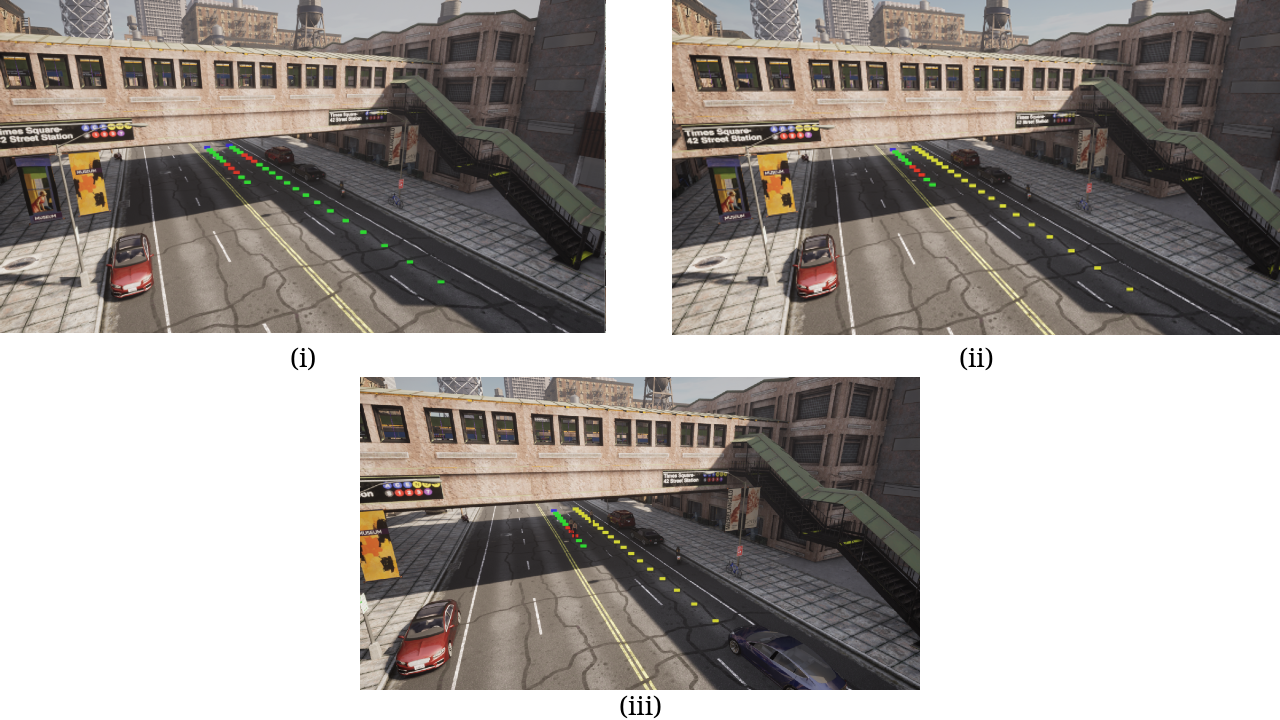
\includegraphics[width=\textwidth]{images/lane-change.png}
  Figure 7: Carla scenario 17
\end{center}

It is inspired by \textit{17 - Obstacle avoidance without prior action} where the vehicle aims to avoid pedestrians whose presence is probabilistic by lane change.

 The right lane has an uncertain subgraph whose distribution is $0.2$, $0.5$, $0.2$. The left lane has an uncertain subgraph whose distribution is $0.7$, $0.8$, $0.8$. The vehicle decided to take the right lane. The results of 10 trials are as follows.

\begin{table}[h]
\centering
\begin{tabular}{cccc}
\toprule
\textbf{Trial} & \textbf{Left Penalty} & \textbf{Right Penalty} & \textbf{Positive} \\
\midrule
1 & 0.33 & 0.5 & \checkmark \\
2 & 0.5 & 0.5 & \ding{55} \\
3 & 0.25 & 0.5 & \checkmark \\
4 & 0.25 & 1.0 & \checkmark \\
5 & 0.25 & 1.0 & \checkmark \\
6 & 0.25 & 0.5 & \checkmark \\
7 & 0.33 & 0.33 & \ding{55} \\
8 & 0.25 & 1.0 & \checkmark \\
9 & 0.33 & 1.0 & \checkmark \\
10 & 0.33 & 0.5 & \checkmark \\
\bottomrule
\end{tabular}
\caption{Left and right lanes' penalties.}
\label{table:3}
\end{table}

As the vehicle is ahead of deciding between two lanes, both lanes decisions are emulated on Carla, where penalty is computed for both. If our mechanism led to a better penalty, i.e higher score, we declare the trial to be positively justifying our decision. In this case, it is reducing collisions with pedestrians. Here $80 \%$ of tested trials are positive.


\textbf{Break}

\begin{center}
  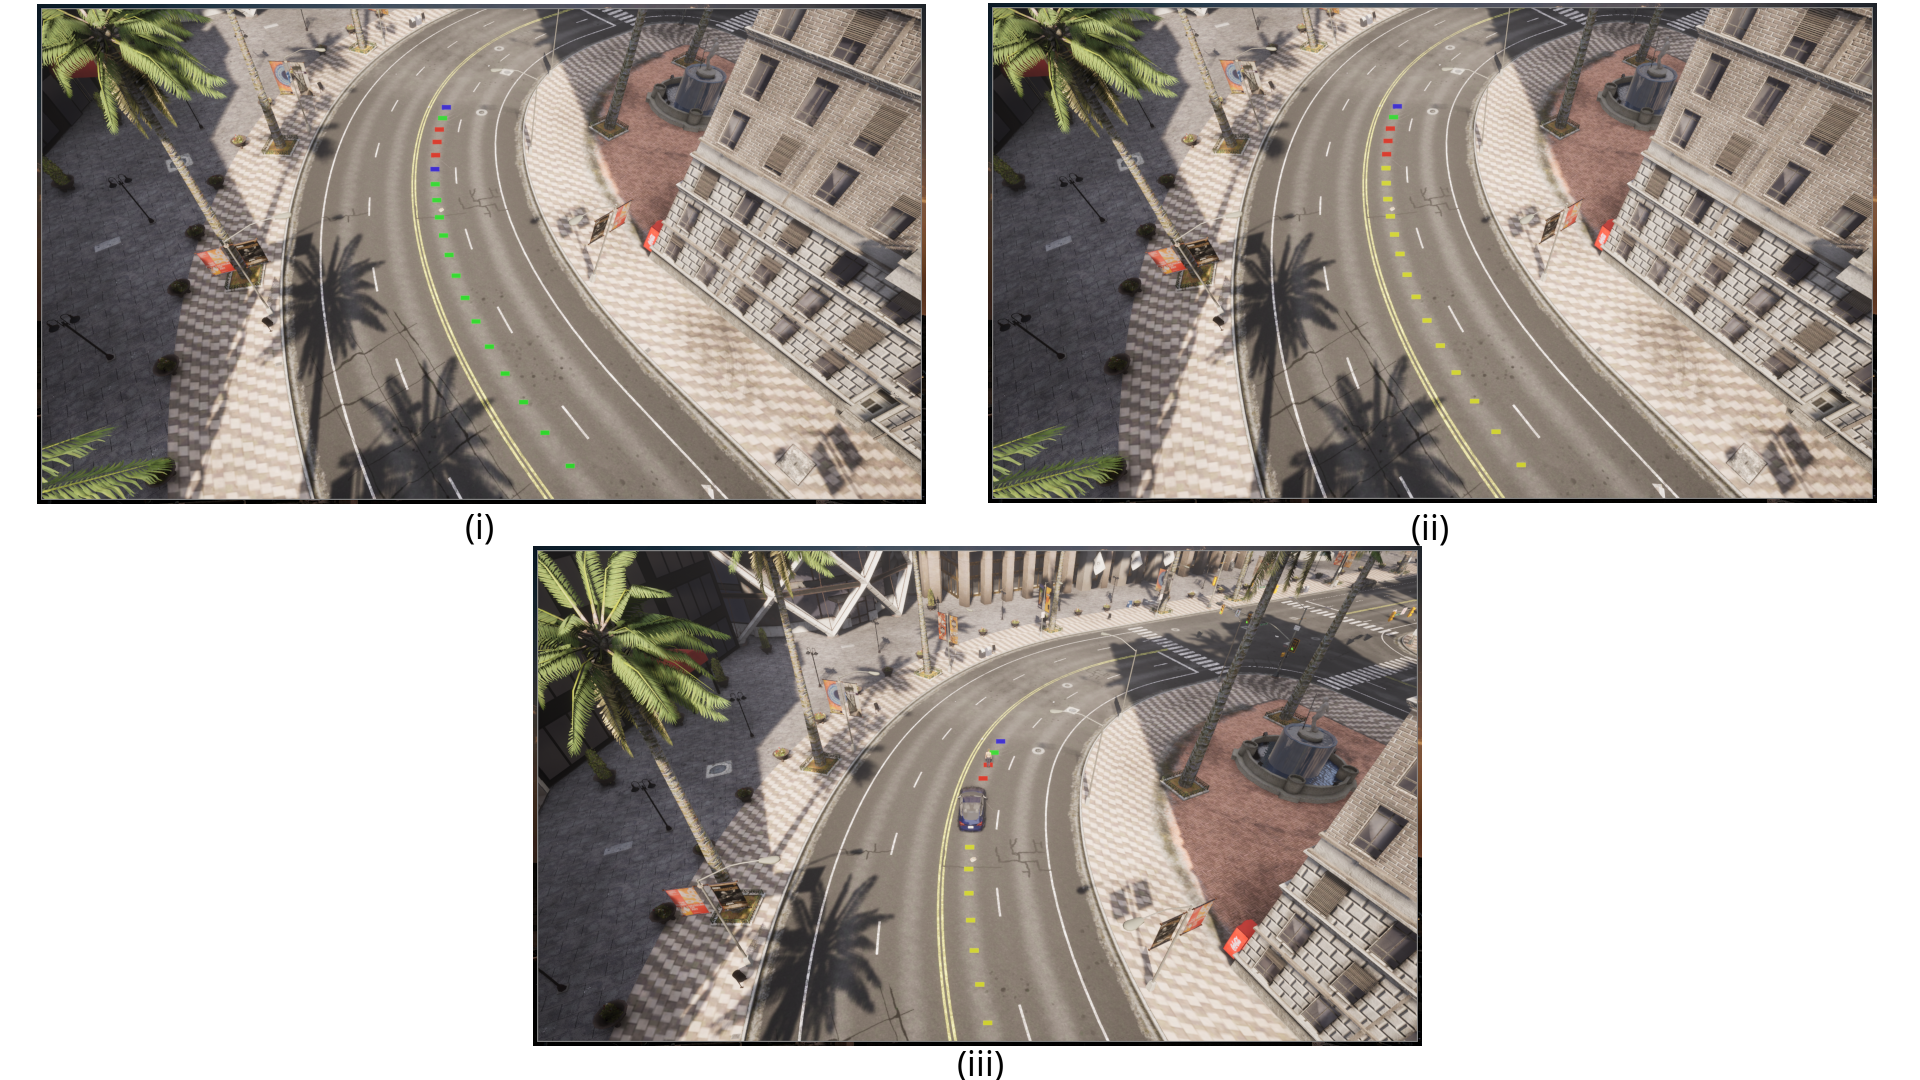
\includegraphics[width=\textwidth]{images/brake.png}
  Figure 8: Carla scenario 16
\end{center}

It is inspired by \textit{16 - Longitudinal control after leading vehicle’s brake} where the vehicle brakes to avoid hitting pedestrians whose presence is probabilistic.

The uncertain subgraph distribution is $0.4, 0.1, 0.7$. The vehicle decided to brake before any uncertain vertex. The results of 10 trials are as follows.

\begin{table}[h]
\centering
\begin{tabular}{cccc}
\toprule
\textbf{Trial} & \textbf{Brake Penalty} & \textbf{Advance Penalty} & \textbf{Positive} \\
\midrule
1 & 0.5 & 0.5 & \ding{55} \\
2 & 1.0 & 0.5 & \checkmark \\
3 & 1.0 & 1.0 & \ding{55} \\
4 & 1.0 & 1.0 & \ding{55} \\
5 & 1.0 & 0.5 & \checkmark \\
6 & 0.5 & 0.5 & \ding{55} \\
7 & 0.5 & 0.33 & \checkmark \\
8 & 1.0 & 0.5 & \checkmark \\
9 & 1.0 & 0.5 & \checkmark \\
10 & 0.5 & 0.33 & \checkmark \\
\bottomrule
\end{tabular}
\caption{Brake versus advance penalties.}
\label{table:4}
\end{table}

As the vehicle is ahead of deciding between braking and advancing, both lanes decisions are emulated on Carla, where penalty is computed for both. We declare a trial to be positive similarly as we did before. In this case, it is reducing collisions with pedestrians. Here $60 \%$ of tested trials are positive.

It is notable to highlight the percentage here is decreased as the vehicle takes some time until it completely stops. Even if it decides to break at a way-point which is safe to be positioned in, acceleration effects may cause it to encroach into the uncertain zone. The odds of that increase if the vehicle is moving faster and an object turns out to be positioned near the boundaries of the uncertain zone.

We analyze how many meters are encroached from the uncertain graph, given distance between the vehicle and the uncertain graph, alongside vehicle's speed, during the moment of braking. In \textit{Image 3} the vehicle brakes only one waypoint, i.e 2 meters, from the uncertain graph colored in red.

\begin{center}
  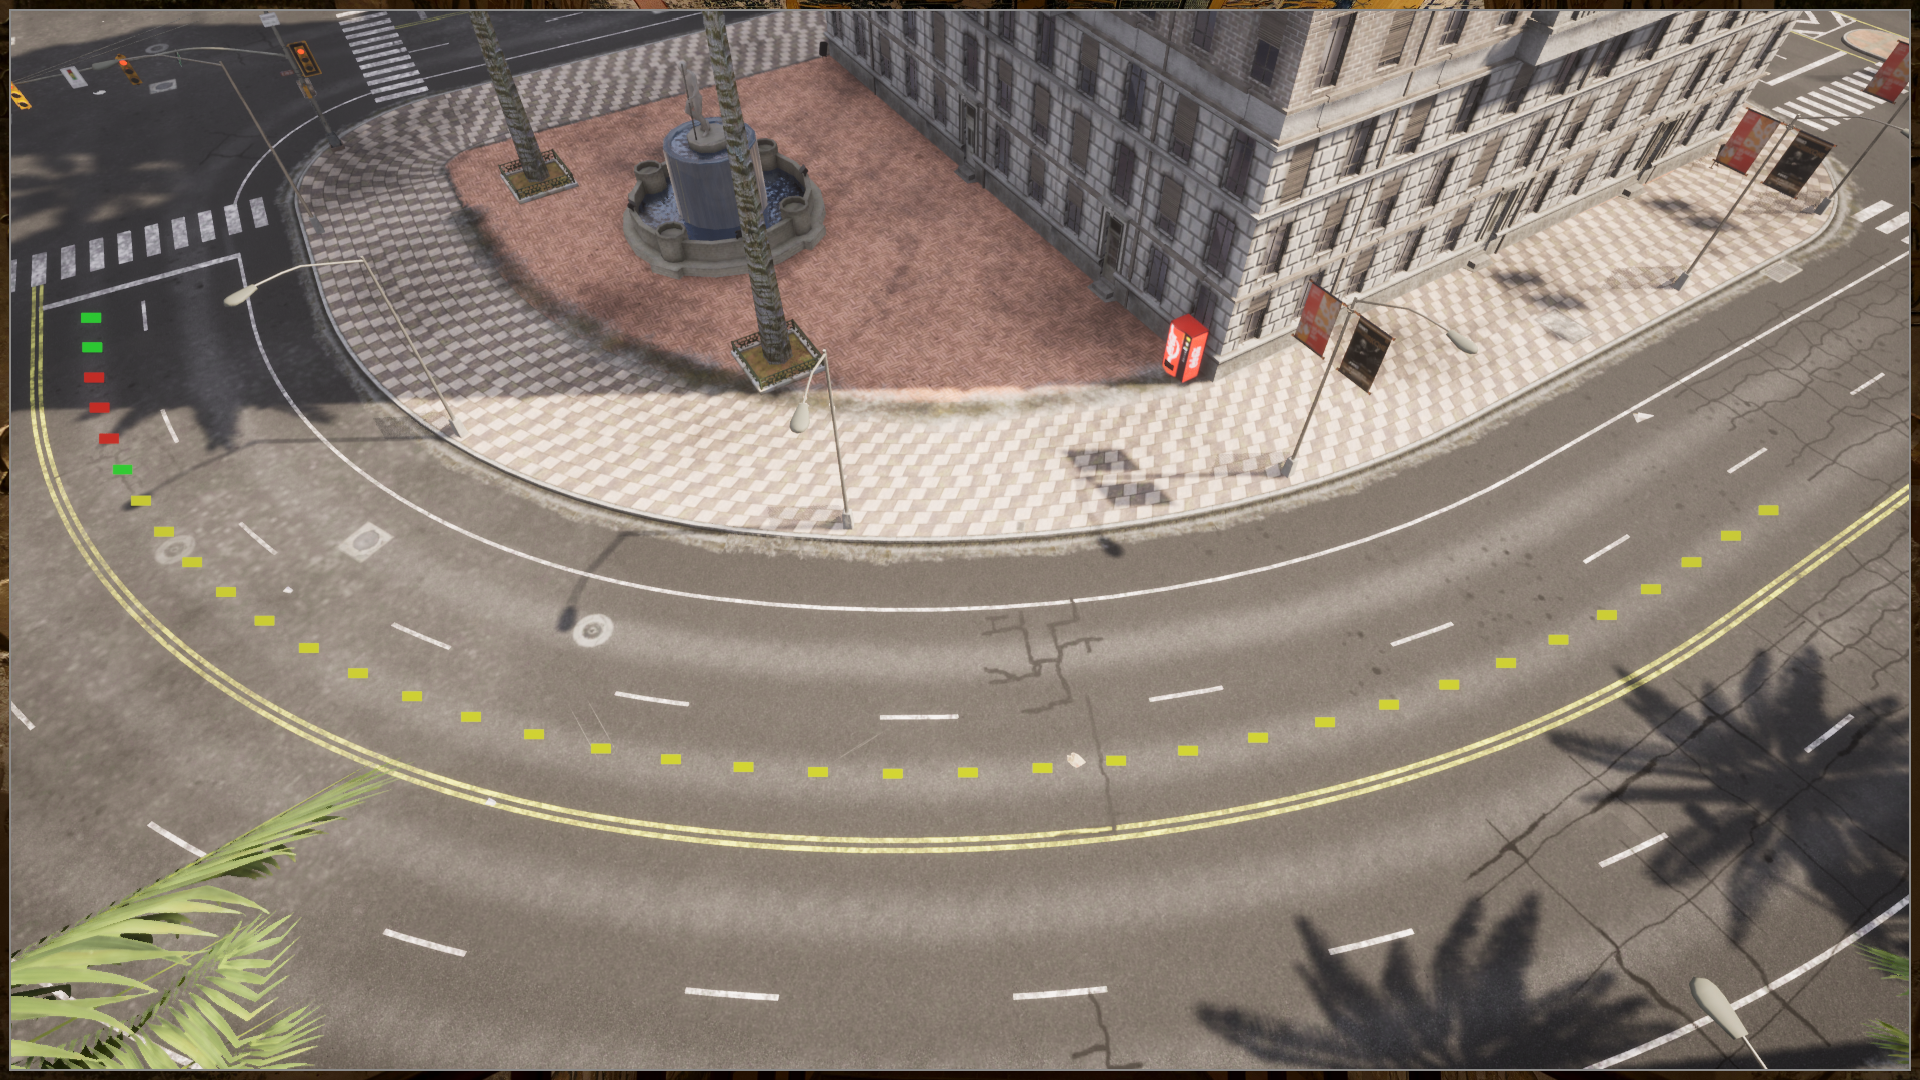
\includegraphics[width=0.5\textwidth]{images/brake-distance.png} \\
  Figure 9: Break analysis
\end{center}

The results of testing multiple values of distances and speeds are in \textit{Table 5}. For example, when the vehicle was 2 meters ahead of the uncertain graph with speed 60 km/h, it encroached 6 meters from the uncertain subgraph.

\begin{table}[h]
\centering
\begin{tabular}{cccc}
\toprule
\multicolumn{1}{c}{\textbf{Distance (m)}} & \multicolumn{3}{c}{\textbf{Speed (km/h)}} \\
\multicolumn{1}{c}{} & \textbf{30} & \textbf{45} & \textbf{60} \\
\midrule
2 & 2 & 4 & 6 \\
4 & 2 & 4 & 4 \\
8 & 0 & 0 & 0 \\
\bottomrule
\end{tabular}
\caption{Meters encroached given distances and speeds.}
\label{table:5}
\end{table}

Results suggest more than 4 meters are needed to avoid the uncertain subgraph upon braking.

In the \textit{Lane Change} scenario, modifying the distance and speed has no notable difference; the vehicle performs lane changes under these modified variables.

\textbf{Intersection}

\begin{center}
  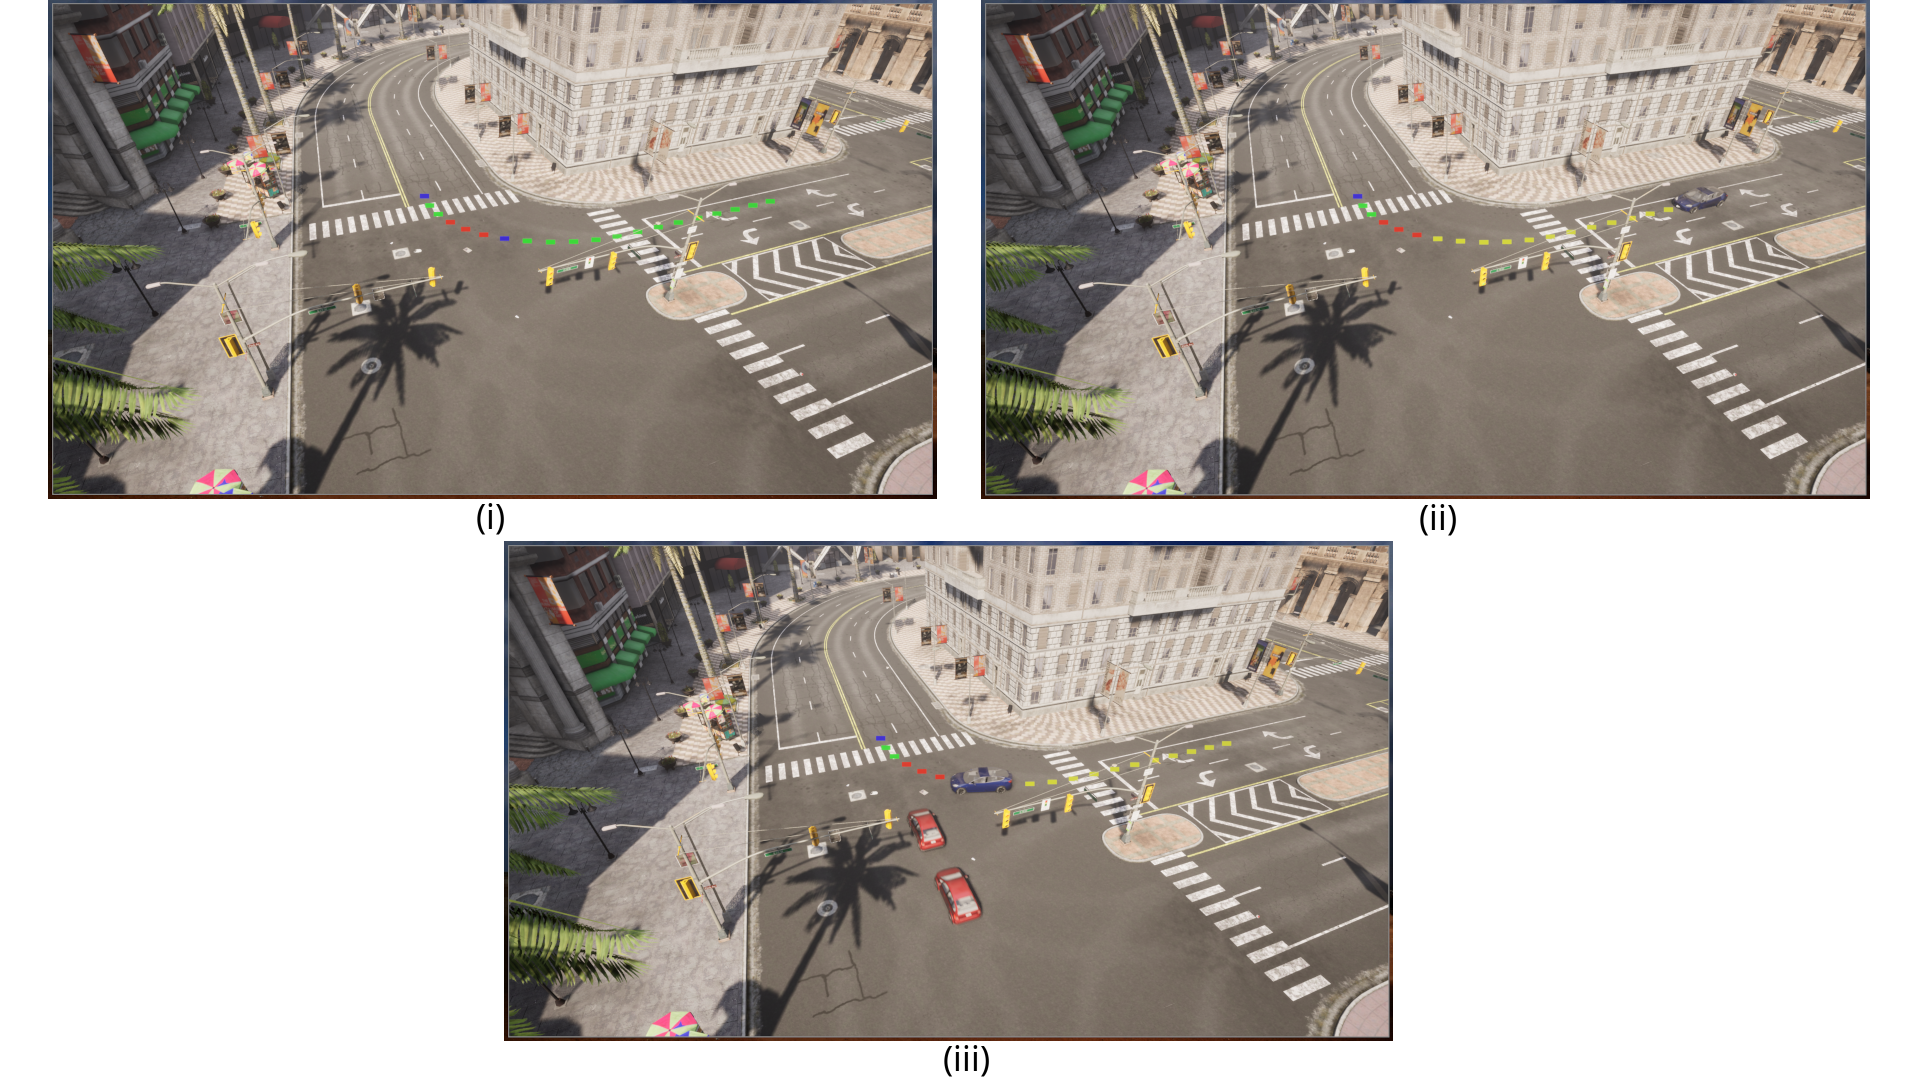
\includegraphics[width=\textwidth]{images/intersection.png}
  Figure 10: Carla scenario 3
\end{center}

It is inspired by \textit{3 - Right turn at an intersection with crossing traffic.} where the vehicle breaks to avoid hitting crossing vehicles whose presence is probabilistic.

The uncertain subgraph distribution is $0.6, 0.5, 0.7$. The vehicle decided not to take the intersection. The results of 10 trials are as follows.

\begin{table}[h]
\centering
\begin{tabular}{cccc}
\toprule
\textbf{Trial} & \textbf{Intersection Penalty} & \textbf{Brake Penalty} & \textbf{Positive} \\
\midrule
1 & 0.59 & 1.0 & \checkmark \\
2 & 0.42 & 1.0 & \checkmark \\
3 & 0.59 & 1.0 & \checkmark \\
4 & 0.59 & 1.0 & \checkmark \\
5 & 0.59 & 1.0 & \checkmark \\
6 & 0.42 & 1.0 & \checkmark \\
7 & 1.0 & 1.0 & \ding{55} \\
8 & 1.0 & 1.0 & \ding{55} \\
9 & 0.42 & 1.0 & \checkmark \\
10 & 0.42 & 1.0 & \checkmark \\
\bottomrule
\end{tabular}
\caption{Brake versus intersecting penalties.}
\label{table:6}
\end{table}

As the vehicle is ahead of deciding between taking the intersection and braking, both decisions are emulated on Carla, where penalty is computed for both. We declare a trial to be positive similarly as we did before. In this case, it is reducing collisions with vehicles. Here $80 \%$ of tested trials are positive.

Observe the percentage here is increased, as the vehicle moves slowly at conjunctions, so it can break confidently.


\section{Conclusion}

We designed a mechanism that enables autonomous vehicles to take a decision under uncertainty. It is independent of any prior environmental knowledge and can be used with any module producing probabilistic information alongside penalties. Computational time is reduced by querying shortest-path only on uncertain zones. Our dynamic update mechanism utilizes computed uncertain subgraphs. The statistical dropout sampling technique was utilized for evaluation. In particular, minimizing probabilistic expectation conforms to the empirically tested trials on Carla emulator.

In this work, we aimed for finding the optimal solution. It may happen that updates are frequent, up to the point where our mechanism has to re-compute everything from scratch. In such case, designing a time-bounded mechanism at the expense of maintaining optimality may be preferred. We suggest to the reading sampling random paths as quick as possible, then improving given the time the vehicle has. Checking \textit{Iterative Methods} may be a good starting point.

\bibliography{ref}

\end{document}
